\chapter{O \textit{firmware} CLEAN}\label{appendix: firmware}

O \textit{firmware} dos dispositivos foi desenvolvido para o microcontrolador Microchip ATMega2560 embarcado em uma plataforma Arduino Mega. O código foi implementado na linguagem de programação C/C++ utilizando o \textit{framework} de Arduino, disponível na IDE PlatformIO para o editor de código Microsoft Visual Studio (VSCode).

Para a programação de todas as funcionalidades do \textit{firmware}, o código foi estruturado em um conjunto de classes. Essa estrutura foi concebida visando seu reaproveitamento em outros microcontroladores suportados no Framework Arduino, como o ESP8266 da Espressif, e também para facilitar a revisão e manutenção do código. As classes desenvolvidas para o projeto estão distribuídas em três pacotes de bibliotecas: o pacote \textit{IoT}, o pacote \textit{Data} e o pacote \textit{Hardware Interfaces}.

O pacote \textit{IoT} encapsula os processos associados à conexão na rede Wi-Fi, comunicação com o servidor e envio de dados pelo protocolo \textit{HTTP}. Já o pacote \textit{Data} engloba todas as funcionalidades relacionadas à preparação dos dados dos sensores para seu armazenamento e transmissão. Este pacote permite abstrair as informações de concentração adquiridos pelos sensores de gases, de detalhes específicos sobre o funcionamento e operação do hardware destes sensores. Ele atua como uma camada intermediária entre as tarefas de aquisição, e as de armazenamento e transmissão dos dados. Por último, o pacote \textit{Hardware Interfaces} agrupa as classes e estruturas utilizadas para interfacear todo o hardware periférico ao microcontrolador utilizado, como sensores, módulos de temporização, módulos de geolocalização e módulos de armazenamento.

\section{Código CLEAN Arduino Mega}

O código consiste em duas partes: uma para configuração (\textit{setup}) e outra para o laço (\textit{loop}) de execução principal. A versão atual do código possui quatro funcionalidades principais que estão de acordo com o hardware do monitor, sendo elas:

\begin{enumerate}
    \item Amostragem, ou leitura das saídas dos sensores
    \item Armazenamento das informações de concentração de gás em um cartão SD
    \item Envio dos dados dos sensores para o servidor Renovar através do microcontrolador ESP8266
    \item Leitura das coordenadas geográficas do local onde ocorre cada leitura
\end{enumerate}

A Figura \ref{fig:fw-main-loop} mostra um fluxograma do código programado para o ATMega2560. Como acontece com todo programa do Arduino Framework, o código é executado em duas funções principais: \texttt{setup()} e \texttt{loop()}. Na versão atual do firmware, o \texttt{setup} prepara a comunicação entre os módulos externos (i.e.: RTC, Wi-Fi, cartão de memória e sensores seriais) e o microcontrolador. A função \texttt{loop()} verifica se o ESP8266 não responde há algum tempo, e, se for o caso, é enviado um sinal RESET para o ESP8266. O resto da função está dividido em quatro seções que são executadas periódicamente e controlam as funcionalidades mencionadas. 

O firmware inclui mais uma funcionalidade que está separada do fluxo principal do programa: a função \texttt{serialEvent3()} que trata os eventos de interrupção da porta serial \texttt{UART3}. Ela é executada cada vez que novos dados são recebidos no \texttt{buffer} dessa interface de hardware que estabelece a comunicação entre o Arduino Mega e o microcontrolador ESP8266. A seguir, são descritas as diferentes seções do código.

\begin{figure}
    \centering
    \caption{Fluxograma do firmware programado para o microcontrolador Arduino MEGA}
    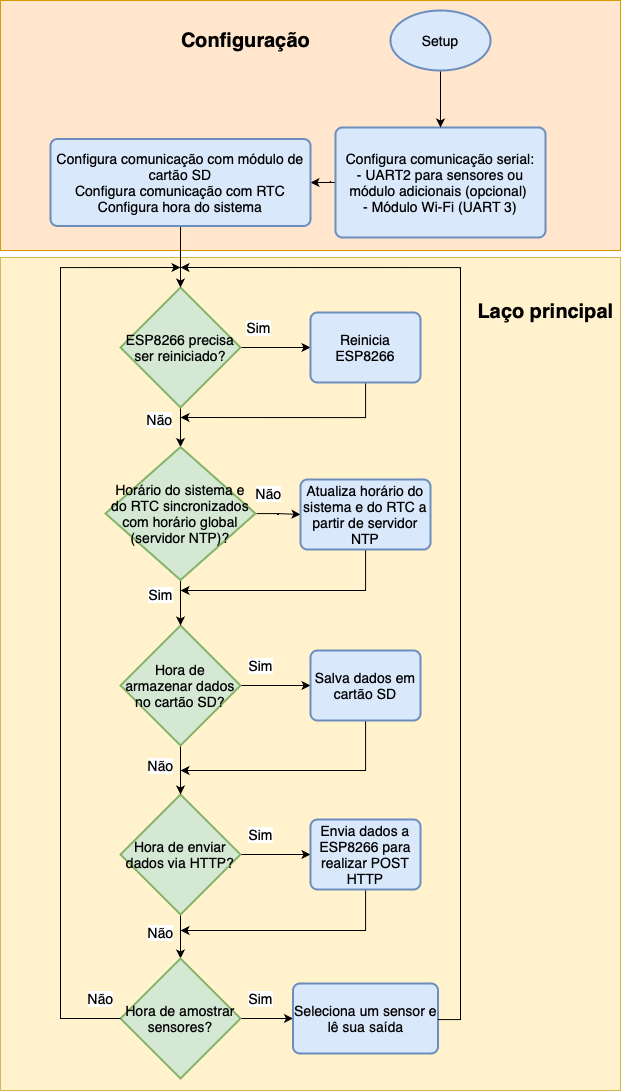
\includegraphics[width=0.5\linewidth]{aftertext//Firmware//Figuras/Main Loop (PT).png}
    \label{fig:fw-main-loop}
    \fonte{Desenvolvido pelo autor (2023)}
\end{figure}

\subsection{Identificação do dispositivo e seus sensores}

Uma parte crucial do firmware é a identificação do dispositivo e dos sensores conectados a ele. Essas identificações deverão corresponder às que tenham sido previamente configuradas no servidor da aplicação Web Renovar, já que serão utilizadas pela aplicação backend para atualizar o banco de dados. A definição do dispositivo é feita na seguinte linha:

\texttt{unsigned long Device::id = <THE NUMBER OF YOUR DEVICE>;}

Depois disso, devem ser definidos os IDs dos sensores, de forma que cada um deles represente uma variável na aplicação Renovar. O código da Lista \ref{code: sensors-ids} exemplifica a definição dos identificadores de 6 sensores previamente registrados na aplicação Renovar. 

\begin{lstlisting}[language=C++, caption=Definição dos identificadores dos sensores de um dispositivo]
    enum iotId_e {      
         // The ID of the CO gas concentration read from a sensor
        CO_ID       = 156,
        // The ID of the NO2 gas concentration read from a sensor
        NO2_ID      = 157, 
        // The ID of the O3 gas concentration  read from a sensor
        O3_ID       = 158,
        // The ID of the SO2 gas concentration  read from a sensor
        SO2_ID      = 159, 
        // The ID of the temperature variable
        TEMP_ID     = 160,
        // The ID of the relative humidity variable
        RHUM_ID     = 161
};
\end{lstlisting}
\label{code: sensors-ids}

\subsection{Configuração: a função \texttt{setup()}}

A função \texttt{setup()} prepara a comunicação entre os módulos externos e o microcontrolador. O código desta função é mostrado na Lista \ref{code: setup-func}. Primeiramente o programa configura as portas seriais que serão utilizadas para comunicação com os sensores seriais utilizando uma interface RS-458 (RS485\_2) e ESP8266 (Serial3). Cada porta serial é inicializada a uma taxa de transmissão previamente definida no código, conforme será descrito posteriormente. A porta serial UART0 (Serial) é usada para depuração. O RS485\_2 implementa uma interface serial ao barramento RS485 que conecta os sensores ao microcontrolador. A função também reinicia o microcontrolador ESP8266 através do objeto \texttt{espIoT}, inicializa as interfaces para o cartão SD e módulos RTC e define a hora do sistema. A continuação são descritos os objetos, constantes e funções usados nesta parte do código.

\begin{lstlisting}[language=C++, caption=Definição dos identificadores dos sensores de um dispositivo]
void setup()
{  
    Serial.begin(9600);
    #ifndef FIXED_DEVICE
    Serial1.begin(GPSBaud);
    #endif
    Serial3.begin(9600UL);
    
    pinMode(13, OUTPUT);
    digitalWrite(13, HIGH);
    
    espIoT.restart();
    
    SD.begin(CHIPSEL_PIN);
    
    Rtc.Begin();
    if (!Rtc.GetIsRunning())
    {
      Rtc.SetIsRunning(true);
    }
    #ifdef DS3231
      Rtc.Enable32kHzPin(false);
      Rtc.SetSquareWavePin(DS3231SquareWavePin_ModeNone);
    #endif
    time_t now = Rtc.GetDateTime().Epoch32Time();
    setSyncProvider(sync_time);
    setSyncInterval(5*SECS_PER_MIN);
    TimeDriver::config(TIMEZONE_SEC);
    SHT20.initSHT20();
    BMP280.begin(BMP280_ADDRESS_ALT, BMP280_CHIPID);
    Alpha_OPC.begin();
    #ifdef FIXED_DEVICE
    GPSDriver::set_coordinates(true, 
                                DeviceFixedLocation::LATITUDE,
                                DeviceFixedLocation::LONGITUDE, 
                                DeviceFixedLocation::ALTITUDE); 
    #endif
    mLastTime = millis();
    mLastTimeGPS = mLastTime;
    mLastTimeuSD = mLastTime;
    mLastTimeHTTP = mLastTime;
}
\end{lstlisting}
\label{code: setup-func}

\subsubsection{\texttt{Serial}, \texttt{Serial1}, \texttt{Serial3}}

Esses objetos, declarados no \textit{framework} Arduino, representam as portas UART do microcontrolador. Os objetos são inicializados pela função \texttt{begin()}, que recebe a taxa de transmissão da comunicação serial. O objeto \texttt{Serial} representa a porta serial \texttt{UART0} que é usada para depuração do programa. Já os objetos \texttt{Serial1} e \texttt{Serial3}, que representam as portas seriais \texttt{UART1} e \texttt{UART3} do Arduino Mega, são utilizadas para comunicação com o módulo GPS e o microcontrolador ESP8266 respectivamente.

A variável \texttt{GPSBaud} é uma constante que define a velocidade em \textit{bits} por segundo da comunicação serial entre o microcontrolador ATMega do Arduino e o módulo GPS. O valor predeterminado é 9600 baúdios, definido na biblioteca \texttt{serial-geo-interface}, mas pode ser redefinido segundo a aplicação. 

\subsubsection{\texttt{espIoT}}

Este é um objeto da classe \texttt{ESPSerialInterface} definido na biblioteca \texttt{serial-internet-interface}. Este objeto controla a comunicação com o ESP8266 conectado ao UART3 do Arduino. A função \texttt{restart()} envia um sinal de \textit{RESET} para o ESP8266. O objeto \texttt{espIoT} é definido no código da seguinte forma: \texttt{ESPSerialInterface espIoT(\&Serial3);}

\subsubsection{\texttt{SD}}

Este é um objeto do \texttt{SDClass} declarado no núcleo do Arduino para interfacear módulos de cartão SD. Ele é inicializado com um método \texttt{begin()} que recebe o pino digital que se conecta ao pino CS do módulo. O pino digital utilizado para a versão atual do hardware e firmware é definido no arquivo \texttt{hardstorage.h} da seguinte forma: \texttt{\#define CHIPSEL\_PIN 53}

\subsubsection{\texttt{Rtc}}

Este é um objeto da classe \texttt{RtcDS3231} definida na biblioteca \texttt{Rtc} de Makuna. O objeto \texttt{Rtc} é declarado da seguinte forma: 

\begin{lstlisting}[language=C++]
    #define I2C Wire
    RtcDS3231<TwoWire> Rtc(I2C);
\end{lstlisting}

 A instância \texttt{Rtc} é inicializada com a função \texttt{begin()} e posteriormente o código verifica se o módulo está funcionando por meio de uma chamada ao método \texttt{GetIsRunning()}. Caso não esteja rodando, o código chama o método \texttt{SetIsRunning(true)}. Caso o módulo \acrshort{rtc} DS3231 tenha sido configurado incorretamente, o código também redefine seu status através do seguinte código: 

\begin{lstlisting}[language=C++]
    #ifdef DS3231
    Rtc.Enable32kHzPin(false);
    Rtc.SetSquareWavePin(DS3231SquareWavePin_ModeNone);
    #endif
\end{lstlisting}

A chamada ao método \texttt{Rtc.GetDateTime().Epoch32Time()} da classe \texttt{RtcDS3231} obtém a hora atual do módulo \acrshort{rtc} no formato UNIX. Já os métodos \texttt{setSyncProvider(getExternalTime getTimeFunction)} e \texttt{setSyncInterval(time\_t interval)} são funções da biblioteca \texttt{Time} que permitem a sincronização automática da hora do sistema com uma fonte de relógio determinada. Neste caso, a fonte utilizada para sincronização é o módulo \acrshort{rtc}. A função \texttt{setSyncProvider()} recebe um ponteiro para uma função que retorna a data e hora atual como uma variável de tipo \texttt{time\_t}. Neste caso, a função que é passada como ponteiro é \texttt{sync\_time()}, declarada anteriormente no código conforme mostrado abaixo: 

\begin{lstlisting}[language=C++]
    RtcDS3231<TwoWire> Rtc(I2C);
    RTCDS3231Interface My_RTCInterface(&Rtc);
    time_t sync_time()  { 
        return RTCDriver<RtcDS3231<TwoWire>>::
            sync_time_from_RTC(&My_RTCInterface);
    }
\end{lstlisting}

A função \texttt{setSyncInterval()} recebe o período de sincronização da hora do sistema, que neste caso foi definido como 5 segundos.

\subsection{Interrupção Serial3}

O código da função que trata a interrupção do UART3 é mostrado na Lista \ref{code: uart3-interruption}. Cada vez que os dados estiverem disponíveis no \textit{buffer} de entrada da porta serial, o objeto \texttt{espIoT} irá analisar a cadeia de catacteres recebida.

\begin{lstlisting}[language=C++, caption=Código para tratamento da interrupção da porta serial UART3]
void serialEvent3() {
    if(Serial3.available()) {
        String buffer = Serial3.readStringUntil(';');
        Serial3.flush();
        espIoT.parse_esp_string(buffer);
    }
}
\end{lstlisting}
\label{code: uart3-interruption}

\subsection{Laço principal do programa: a função \texttt{loop()}}

A sequência de instruções do programa da placa CLEAN Arduino Mega é executado dentro de um laço infinito definido na função \texttt{loop()} do \textit{Framework} Arduino. Esta função é responsável por tratar quatro funcionalidades que foram mencionadas anteriormente, i.e.: amostragem, armazenamento, envio de dados e geolocalização. A Lista \ref{code:main-loop} mostra o código da função \texttt{loop()}.

\begin{lstlisting}[language=C++, caption=Código do laço de execução do programa]
void loop()
{
  static bool sd_ok = false;

  espIoT.watch_dog();
  
  if((!TimeDriver::_already_up_to_date()))  espIoT.request_time();
  if((!My_RTCInterface.is_up_to_date()))    
    RTCDriver<RtcDS3231<TwoWire>>::update_rtc(&My_RTCInterface, now());
  
  
  // /*
  if ((millis() - mLastTime) >= SAMPLE_ITERATION_PERIOD_MS)
  {
    mLastTime = millis();
    static uint8_t index  = 0;
    Vars[index]->smooth(sensors[index]->read());
    index = (index >= numSensors - 1) ? 0 : index + 1;
  }
  // */
  
  // /*
  if((millis() - mLastTimeuSD) >= uSD_TIME_MSEC)
  {
    mLastTimeuSD = millis();
    static uint8_t data_index_uSD = 0;
    Vars[data_index_uSD]->sense(&data);
    
    char* filename = (char*)malloc(strlen_P(
                        filenames[data_index_uSD])+1);
    strcpy_P(filename, filenames[data_index_uSD]);
    if(open_file(filename)) 
      sd_ok = save_to_file(&data, filename);
    else  SD.begin(CHIPSEL_PIN);
    free(filename);
  
    data_index_uSD = (data_index_uSD >= numSensors-1) ? 0 : 
                        data_index_uSD + 1;
  }
  // */
  
  // /*
  if((millis() - mLastTimeHTTP) >= HTTP_TIME_MSEC)
  {
    mLastTimeHTTP = millis();
    static uint8_t data_index_iot = 0;

    Vars[data_index_iot]->sense(&data);
    readings[0] = &data;
    if(!espIoT.send_http_post(&data))  print_debug("Couldn't post!");
    data_index_iot = (data_index_iot >= numSensors-1) ? 0 : 
                        data_index_iot + 1;
  }
  // */
  
  // /*
  if((millis() - mLastTimeGPS) >= MSECS_GPSOUTDATE)
  {
    static uint8_t gps_tries = 0;
    print_debug("[MAIN] GPS");
    mLastTimeGPS = millis();
    if (!gps.read_gps(MSECS_GPSOUTDATE/2))
    {
      if (gps_tries++ > 7)
      {
        GPSDriver::set_coordinates(true,
                                    DeviceDefaultLocation::LATITUDE, 
                                    DeviceDefaultLocation::LONGITUDE, 
                                    DeviceDefaultLocation::ALTITUDE);
        gps_tries = 8;
      }
    }
    else {
      gps_tries = 0;
    }
  }
  // */
}
\end{lstlisting}
\label{code:main-loop}

As quatro funcionalidades principais que o código executa periodicamente são controladas pelas variáveis \texttt{mLastTime}, \texttt{mLastTimeGPS}, \texttt{mLastTimeuSD} e \texttt{mLastTimeHTTP}, que armazenam a marca o instante de tempo em que cada funcionalidade é executada. As constantes \texttt{uSD\_TIME\_MSEC}, \texttt{HTTP\_TIME\_SEC}, \texttt{SAMPLE\_ITERATION\_PERIOD\_MS} e \texttt{MSECS\_GPSOUTDATE} representam os períodos em que cada funcionalidade deve ser executada, conforme está resumido na Tabela \ref{tab:seq-main-clean}. Em cada ciclo do laço, o objeto \texttt{espIoT} chama ao método \texttt{watch\_dog()} para verificar se existe alguma solicitação enviada ao ESP8266 cujo tempo de espera tenha expirado. Caso isso aconteça, o ESP8266 será reiniciado. A função \texttt{loop()} também verifica se o microcontrolador atualizou seu horário a partir de um servidor de data e hora da Internet, caso contrário, uma solicitação é enviada ao ESP8266 para retornar o horário atual da Internet.

\begin{table}[h]
    \centering
    \caption{Constantes e variáveis utilizadas para controlar a execução de cada funcionalidade no firmware}
    \label{tab:seq-main-clean}
    \begin{tabularx}{0.98\textwidth}[h]{
         >{\raggedright\hsize=.70\hsize\arraybackslash}X
         >{\raggedright\hsize=.45\hsize\arraybackslash}X 
         >{\raggedright\arraybackslash}X
         >{\raggedleft\arraybackslash}X }
         \hline
        \textbf{Funcionalidade} & \textbf{Período}  & \textbf{Constante definida no código} & \textbf{Variável de controle} \\
        \hline
        Amostragem & 6 segundos & \texttt{SAMPLE\_ITERATION\_PERIOD\_MS} & \texttt{mLastTime} \\
        \hline
        Armazenamento & 60 segundos & \texttt{uSD\_TIME\_MSEC} & \texttt{mLastTimeuSD} \\
        \hline
        Envio de dados & 60 segundos & \texttt{HTTP\_TIME\_MSEC} & \texttt{mLastTimeHTTP} \\
        \hline
        Geolocalização & 70 segundos & \texttt{MSECS\_GPSOUTDATE} & \texttt{mLastTimeGPS} \\
        \hline
    \end{tabularx}
    \fonte{Desenvolvido pelo autor (2023)}
\end{table}

O código também verifica se o módulo \acrshort{rtc} foi atualizado com o horário da internet. Caso contrário, ele chama o método \texttt{update\_rtc()} da classe \texttt{RTCDriver}. Esta classe é um \textit{template} para controlar as funcionalidades relacionadas a um módulo \acrshort{rtc} genérico, como atualizar seu horário, por exemplo. O método \texttt{update\_rtc()} recebe um ponteiro para uma instância da classe \texttt{RTCInterface}, que cria uma interface para o hardware de qualquer módulo \acrshort{rtc}. \texttt{RTCInterface} é uma classe abstrata, portanto, para instanciar essa interface em um módulo \acrshort{rtc}, uma classe concreta deve ser herdada dele. No presente caso, esta instância foi implementada no objeto \texttt{My\_RTCInterface}, declarado previamente no código conforme mostrado abaixo.

\begin{lstlisting}[language=C++]
class RTCDS3231Interface : public RTCInterface<RtcDS3231<TwoWire>>
{
    public:
    RTCDS3231Interface(RtcDS3231<TwoWire>* rtc) : 
    RTCInterface<RtcDS3231<TwoWire>>(rtc) {}
    
    virtual void set_time(time_t t) {
        RtcDateTime dt;
        dt.InitWithEpoch32Time(t);
        _rtc->SetDateTime(dt);
    }
    
    virtual time_t get_time() {
        return _rtc->GetDateTime().Epoch32Time();
    }
};

#define I2C Wire
RtcDS3231<TwoWire> Rtc(I2C);
RTCDS3231Interface My_RTCInterface(&Rtc);
\end{lstlisting}

Como pode ser observado, a classe \texttt{RTCDS3231Interface} herda de \texttt{RTCInterface}. Quando o objeto daquela classe é declarado, ele recebe em seu construtor uma referência a um objeto \texttt{rtc}, que neste caso representa o próprio módulo DS3231. Resumindo, o objeto \texttt{rtc} representa o módulo DS3231; o objeto \texttt{My\_RTCInterface} implementa a interface entre o módulo \acrshort{rtc} e o código principal; e a classe \texttt{RTCDriver} controla as funcionalidades do módulo dentro do código. Essa relação é representada no diagrama da Figura \ref{fig:rtc-classes}.

\begin{figure}[h]
    \centering
    \caption{Módulos e interfaces usados para controle e interface do RTC}
    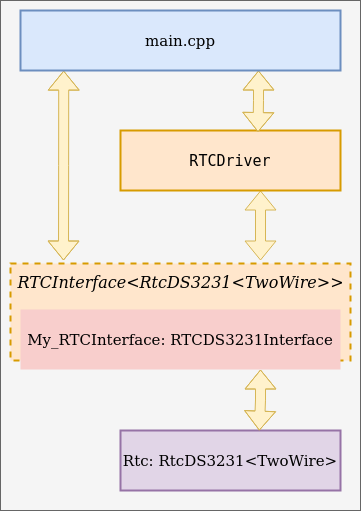
\includegraphics[width=0.5\textwidth]{aftertext/Firmware/Figuras/Diagrama-de-modulos-RTC.png}
    \fonte{Desenvolvido pelo autor (2023)}
    \label{fig:rtc-classes}
\end{figure}

\subsubsection{Leitura dos sensores}

A seção do código que lê os sensores de gás é mostrada na Lista \ref{code:main-read-sensors}. O código primeiro verifica se o tempo de leitura dos sensores já passou e atualiza a variável \texttt{mLastTime}. Esta seção do código basicamente itera entre as listas \texttt{Vars} e \texttt{sensors} para obter a leitura de cada sensor e atribuir a variável correspondente. A lista \texttt{sensors} contém todos os sensores conectados na placa CLEAN, já a lista \texttt{Vars} contém as variáveis que cada sensor representa; um representa a camada de \textit{hardware} enquanto o outro representa uma camada de mais alto nível dos dados, as variáveis físicas. Dessa forma a informação de mais baixo nível contida no sinal de saída dos sensores é transportada para camadas de dados superios que possibilita seu armazenamento e transmissão remota. Na Lista \ref{code:sensors-and-vars} ilustra-se o código que implementa cada uma das listas.

\begin{lstlisting}[language=C++, caption=Código para leitura dos sensores]
if ((millis() - mLastTime) >= SAMPLE_ITERATION_PERIOD_MS)
{
    mLastTime = millis();
    static uint8_t index  = 0;
    Vars[index]->smooth(sensors[index]->read());
    index = (index >= numSensors - 1) ? 0 : index + 1;
}
\end{lstlisting}
\label{code:main-read-sensors}

\begin{lstlisting}[language=C++, caption=Declaração das listas de sensores e variáveis]
Sensor* sensors[numSensors] = 
{
    (SensorInterface<Adafruit_BMP280>*)&IntTempSensor,
    (SensorInterface<Adafruit_BMP280>*)&IntPresSensor,
    (SensorInterface<AlphaSenseCompensator>*)
        (new AlphaSenseCompensatorSensor(&Alpha_COComp)),
    (SensorInterface<AlphaSenseCompensator>*)
        (new AlphaSenseCompensatorSensor(&Alpha_NO2Comp)),
    (SensorInterface<AlphaSenseCompensator>*)
        (new AlphaSenseCompensatorSensor(&Alpha_SO2_1_Comp)),
    (SensorInterface<AlphaSenseCompensator>*)
        (new AlphaSenseCompensatorSensor(&Alpha_O3_1_Comp)),
    (SensorInterface<AlphaSenseCompensator>*)
        (new AlphaSenseCompensatorSensor(&Alpha_O3_2_Comp)),
    (SensorInterface<AlphaSenseCompensator>*)
        (new AlphaSenseCompensatorSensor(&Alpha_SO2_2_Comp)),
    (SensorInterface<DFRobot_SHT20>*)&ExtTempSensor,
    (SensorInterface<DFRobot_SHT20>*)&ExtHumSensor,
    (SensorInterface<AlphasenseOPC>*)(new 
        AlphaSenseOPCPM10Sensor(&Alpha_OPC)),
    (SensorInterface<AlphasenseOPC>*)(new 
        AlphaSenseOPCPM2_5Sensor(&Alpha_OPC)),
    (SensorInterface<AlphasenseOPC>*)(new 
        AlphaSenseOPCPM1Sensor(&Alpha_OPC)),
    (SensorInterface<AlphasenseOPC>*)(new 
        AlphaSenseOPCTempSensor(&Alpha_OPC)),
    (SensorInterface<AlphasenseOPC>*)(new 
        AlphaSenseOPCHumSensor(&Alpha_OPC))
};

Variable* Vars[numSensors] = 
{ 
    new Temperature(TEMPERATURE_ID, SI_TEMP_Celsius, BUFFER_SIZE),
    new Pressure(PRESSURE_ID, SI_PRES_Pascal, BUFFER_SIZE),
    new GasConcentration(ALPHA_CO_ID, SI_CONC_ppb, BUFFER_SIZE),
    new GasConcentration(ALPHA_NO2_ID, SI_CONC_ppb, BUFFER_SIZE),
    new GasConcentration(ALPHA_SO2_1_ID, SI_CONC_ppb, BUFFER_SIZE),
    new GasConcentration(ALPHA_OX_1_ID, SI_CONC_ppb, BUFFER_SIZE),
    new GasConcentration(ALPHA_OX_2_ID, SI_CONC_ppb, BUFFER_SIZE),
    new GasConcentration(ALPHA_SO2_2_ID, SI_CONC_ppb, BUFFER_SIZE),
    new Temperature(EXT_TEMPERATURE_ID, SI_TEMP_Celsius, BUFFER_SIZE),
    new Humidity(EXT_HUMIDITY_ID, SI_HUMD_Relative, BUFFER_SIZE),
    new GasConcentration(PM10_ID, SI_CONC_ug, BUFFER_SIZE),
    new GasConcentration(PM25_ID, SI_CONC_ug, BUFFER_SIZE),
    new GasConcentration(PM01_ID, SI_CONC_ug, BUFFER_SIZE),
    new Temperature(OPC_TEMPERATURE_ID, SI_TEMP_Celsius, BUFFER_SIZE),
    new Humidity(OPC_HUMIDITY_ID, SI_HUMD_Relative, BUFFER_SIZE)
};
\end{lstlisting}
\label{code:sensors-and-vars}

\subsubsection{Armazenamento dos dados}

A seção do código que armazena os dados em um cartão SD é mostrada na Lista . O código primeiro verifica se o tempo de armazenamento dos dados já passou e atualiza a variável \texttt{mLastTimeuSD}. Esta seção do código transfere os dados de cada variável para um objeto \texttt{data}, que é do tipoe \texttt{SensorData} e que é usado para armazenar as informações da variável. O método utilizado para transferir as informações de \texttt{Variable} para \texttt{SensorData} é a função \texttt{sense()}, que recebe um ponteiro para \texttt{SensorData}. Este objeto \texttt{data} é definido anteriormente no código conforme mostrado abaixo. Depois que os dados forem transferidos para a instância de \texttt{SensorData}, eles são armazenados em um arquivo no cartão SD.

\begin{lstlisting}[language=C++, caption=Sequência de armazenamento de dados]
SensorData data;

//...

void loop()
{
  // ...
  if((millis() - mLastTimeuSD) >= uSD_TIME_MSEC)
  {
    mLastTimeuSD = millis();
    static uint8_t data_index_uSD = 0;
    Vars[data_index_uSD]->sense(&data);
    
    char* filename = (char*)malloc(strlen_P(
                        filenames[data_index_uSD])+1);
    strcpy_P(filename, filenames[data_index_uSD]);
    if(open_file(filename)) 
      sd_ok = save_to_file(&data, filename);
    else  SD.begin(CHIPSEL_PIN);
    free(filename);
  
    data_index_uSD = (data_index_uSD >= numSensors-1) ? 0 : 
                        data_index_uSD + 1;
  }
  // ...
}
\end{lstlisting}

\subsubsection{Envio de dados via protocolo \textit{HTTP}}

A seção do código que envia os dados ao ESP8266 para postagem em um servidor HTTP é mostrada abaixo . Assim como as demais seções do código, esta seção primeiro verifica se o tempo de envio dos dados já passou e atualiza a variável \texttt{mLastTimeHTTP}. Depois disso, ele utiliza o último objeto \texttt{SensorData} armazenado para enviar as informações adquiridas para a variável correspondente. O objeto \texttt{espIoT} enviará uma cadeia de caracteres com um objeto \acrshort{json} contendo as informações a serem postadas pelo ESP8266. O método \texttt{send\_http\_post()} recebe um ponteiro para um \texttt{DataContainer}. Como a classe \texttt{SensorData} herda de \texttt{DataContainer}, cada item nos dados pode ser convertido em um ponteiro desse tipo

\begin{lstlisting}
if((millis() - mLastTimeHTTP) >= HTTP_TIME_MSEC)
{
    mLastTimeHTTP = millis();
    static uint8_t data_index_iot = 0;
    
    Vars[data_index_iot]->sense(&data);
    readings[0] = &data;
    if(!espIoT.send_http_post(&data))  print_debug("Couldn't post!");
    data_index_iot = (data_index_iot >= numSensors-1) ? 0 : 
                        data_index_iot + 1;
}
\end{lstlisting}

\subsubsection{Geolocalização}

Por fim, a continuação mostra a seção de código que atualiza as informações de geolocalização do módulo \acrshort{gps}. Assim como nas outras seções do código, esta seção primeiro verifica se passou o tempo para atualizar as informações do \acrshort{gps} e atualiza a variável \texttt{mLastTimeGPS}. Para ler o módulo \acrshort{gps}, o objeto \texttt{gps} invoca o método \texttt{readGPS()}. Este método toma como parâmetro o tempo máximo que o Arduino deve aguardar uma resposta do módulo \acrshort{gps}, neste caso \texttt{MSECS\_GPSOUTDATE/2}. O objeto \texttt{gps} é uma instância da classe \texttt{TinyGPSSerialInterface} que está previamente definida no código conforme mostrado. O construtor deste objeto recebe uma referência à porta serial utilizada para comunicação com o módulo, neste caso \texttt{Serial1}. Em caso de falha na comunicação com o módulo \acrshort{gps}, depois da sétima tentativa, é setado um valor padrão previamente configurado.

\begin{lstlisting}
TinyGPSSerialInterface gps(&Serial1);

//...

void loop()
{
    //...
    
    if((millis() - mLastTimeGPS) >= MSECS_GPSOUTDATE)
    {
        static uint8_t gps_tries = 0;
        print_debug("[MAIN] GPS");
        mLastTimeGPS = millis();
        if (!gps.read_gps(MSECS_GPSOUTDATE/2))
        {
          if (gps_tries++ > 7) {
            GPSDriver::set_coordinates(
                true,
                DeviceDefaultLocation::LATITUDE,
                DeviceDefaultLocation::LONGITUDE, 
                DeviceDefaultLocation::ALTITUDE);
            gps_tries = 8;
          }
        }
        else {
          gps_tries = 0;
        }
    }
}
\end{lstlisting}